\section*{Mini Machine Problem 2 }


\textbf{Answers} 

\begin{enumerate}
\item[1.]  
When $max = 1$, what we do is just to do the exact match. That means each name will match to itself. And the match will always be one. When $max = 0.99$, we are tring to match those names that are similar but not exactly the same. 

 \begin{figure}[H]
  \centering
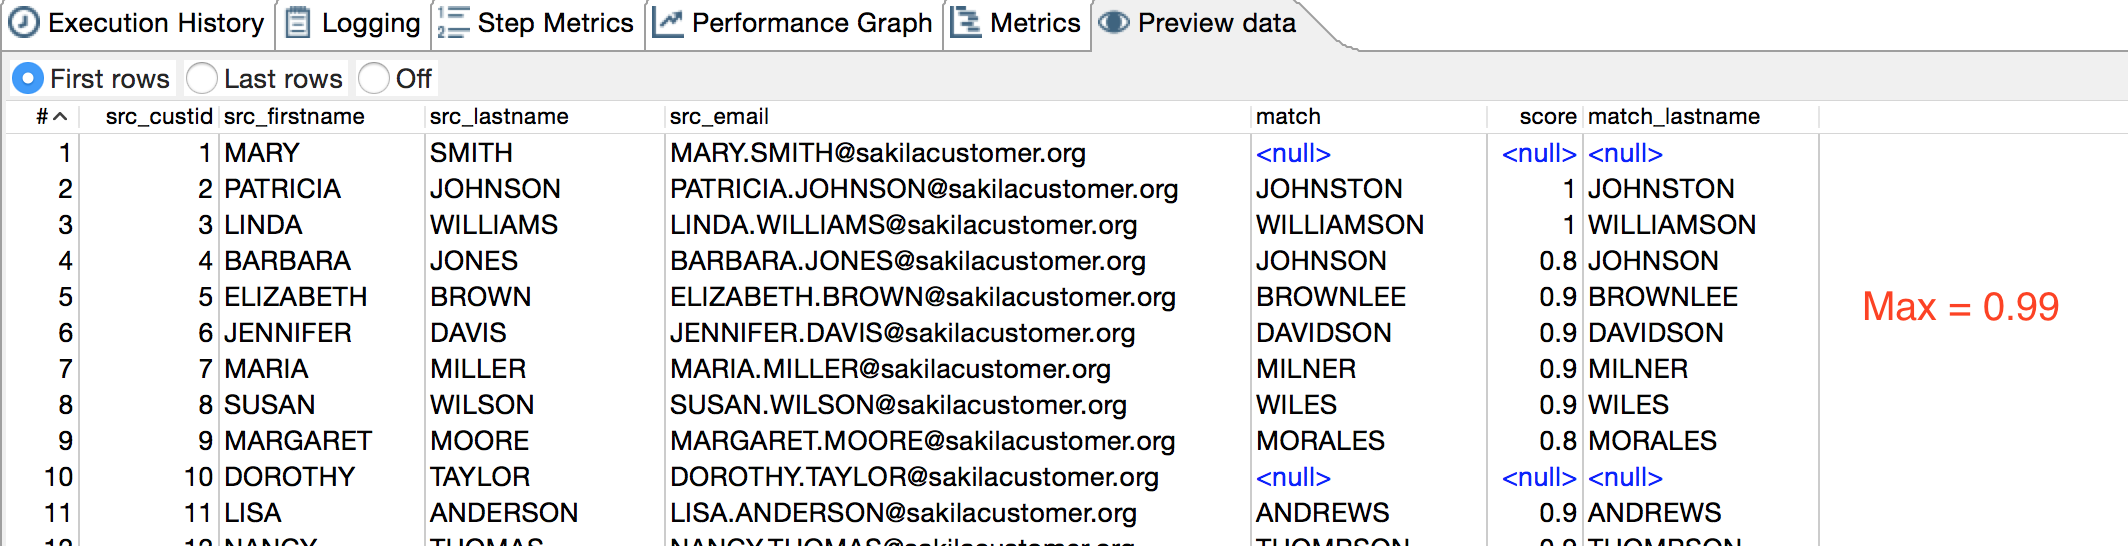
\includegraphics[width=12cm, height=5cm]{max99}
  \end{figure}
  
   \begin{figure}[H]
  \centering
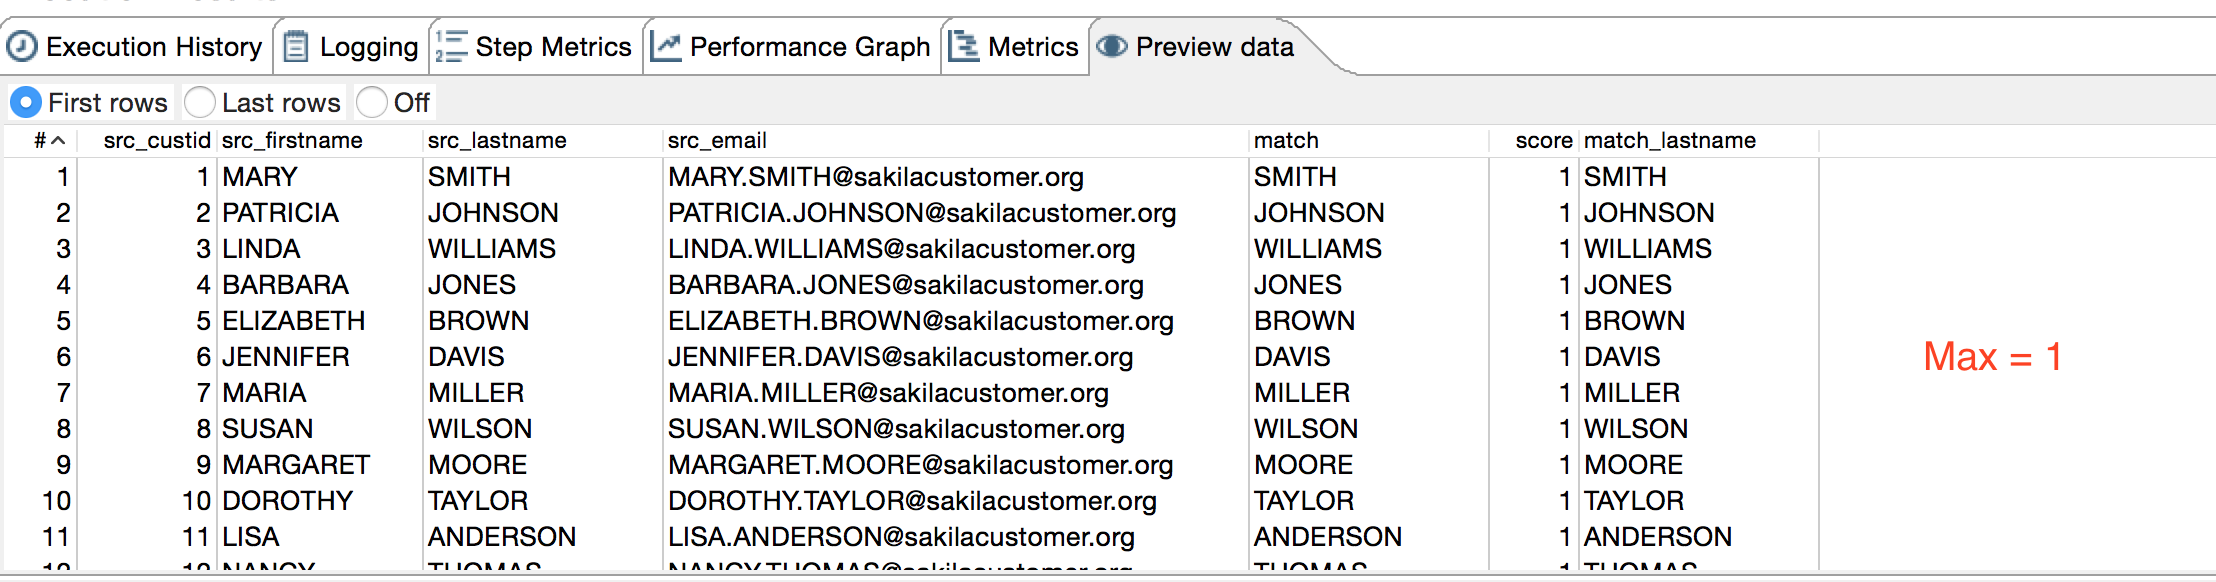
\includegraphics[width=12cm, height=5cm]{max1}
  \end{figure}

\\

\item[2.] 
 \begin{figure}[H]
  \centering
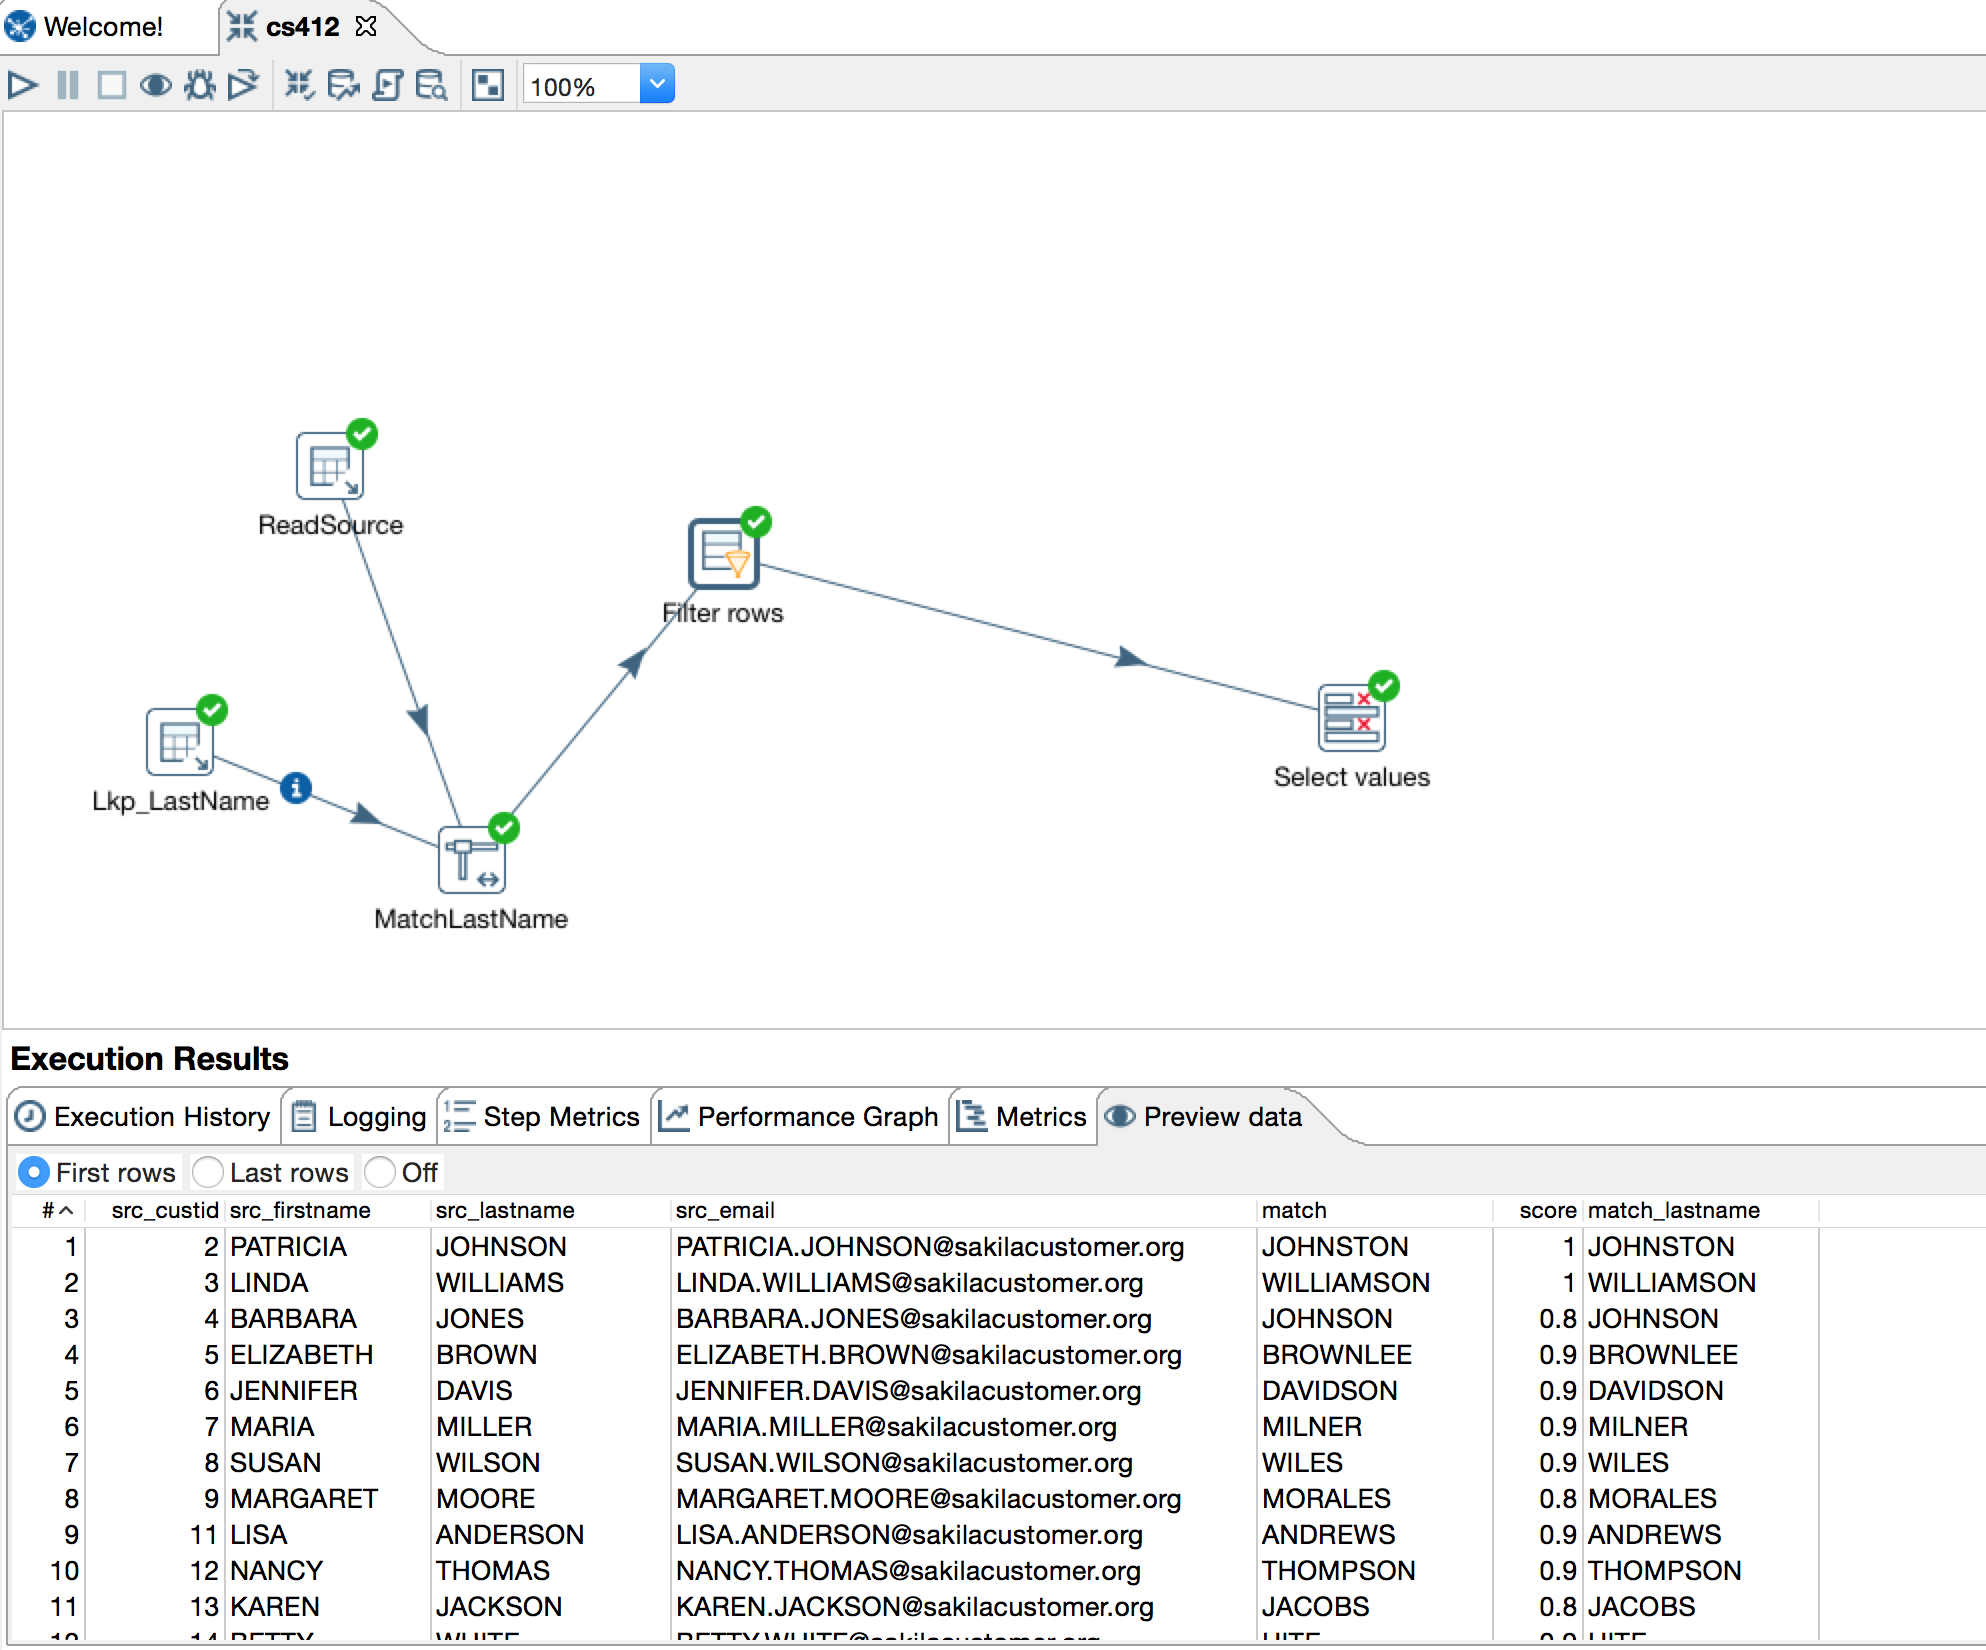
\includegraphics[width=10cm, height=10cm]{mp22}
  \end{figure}
\\

\item[3.] 

 \begin{figure}[H]
  \centering
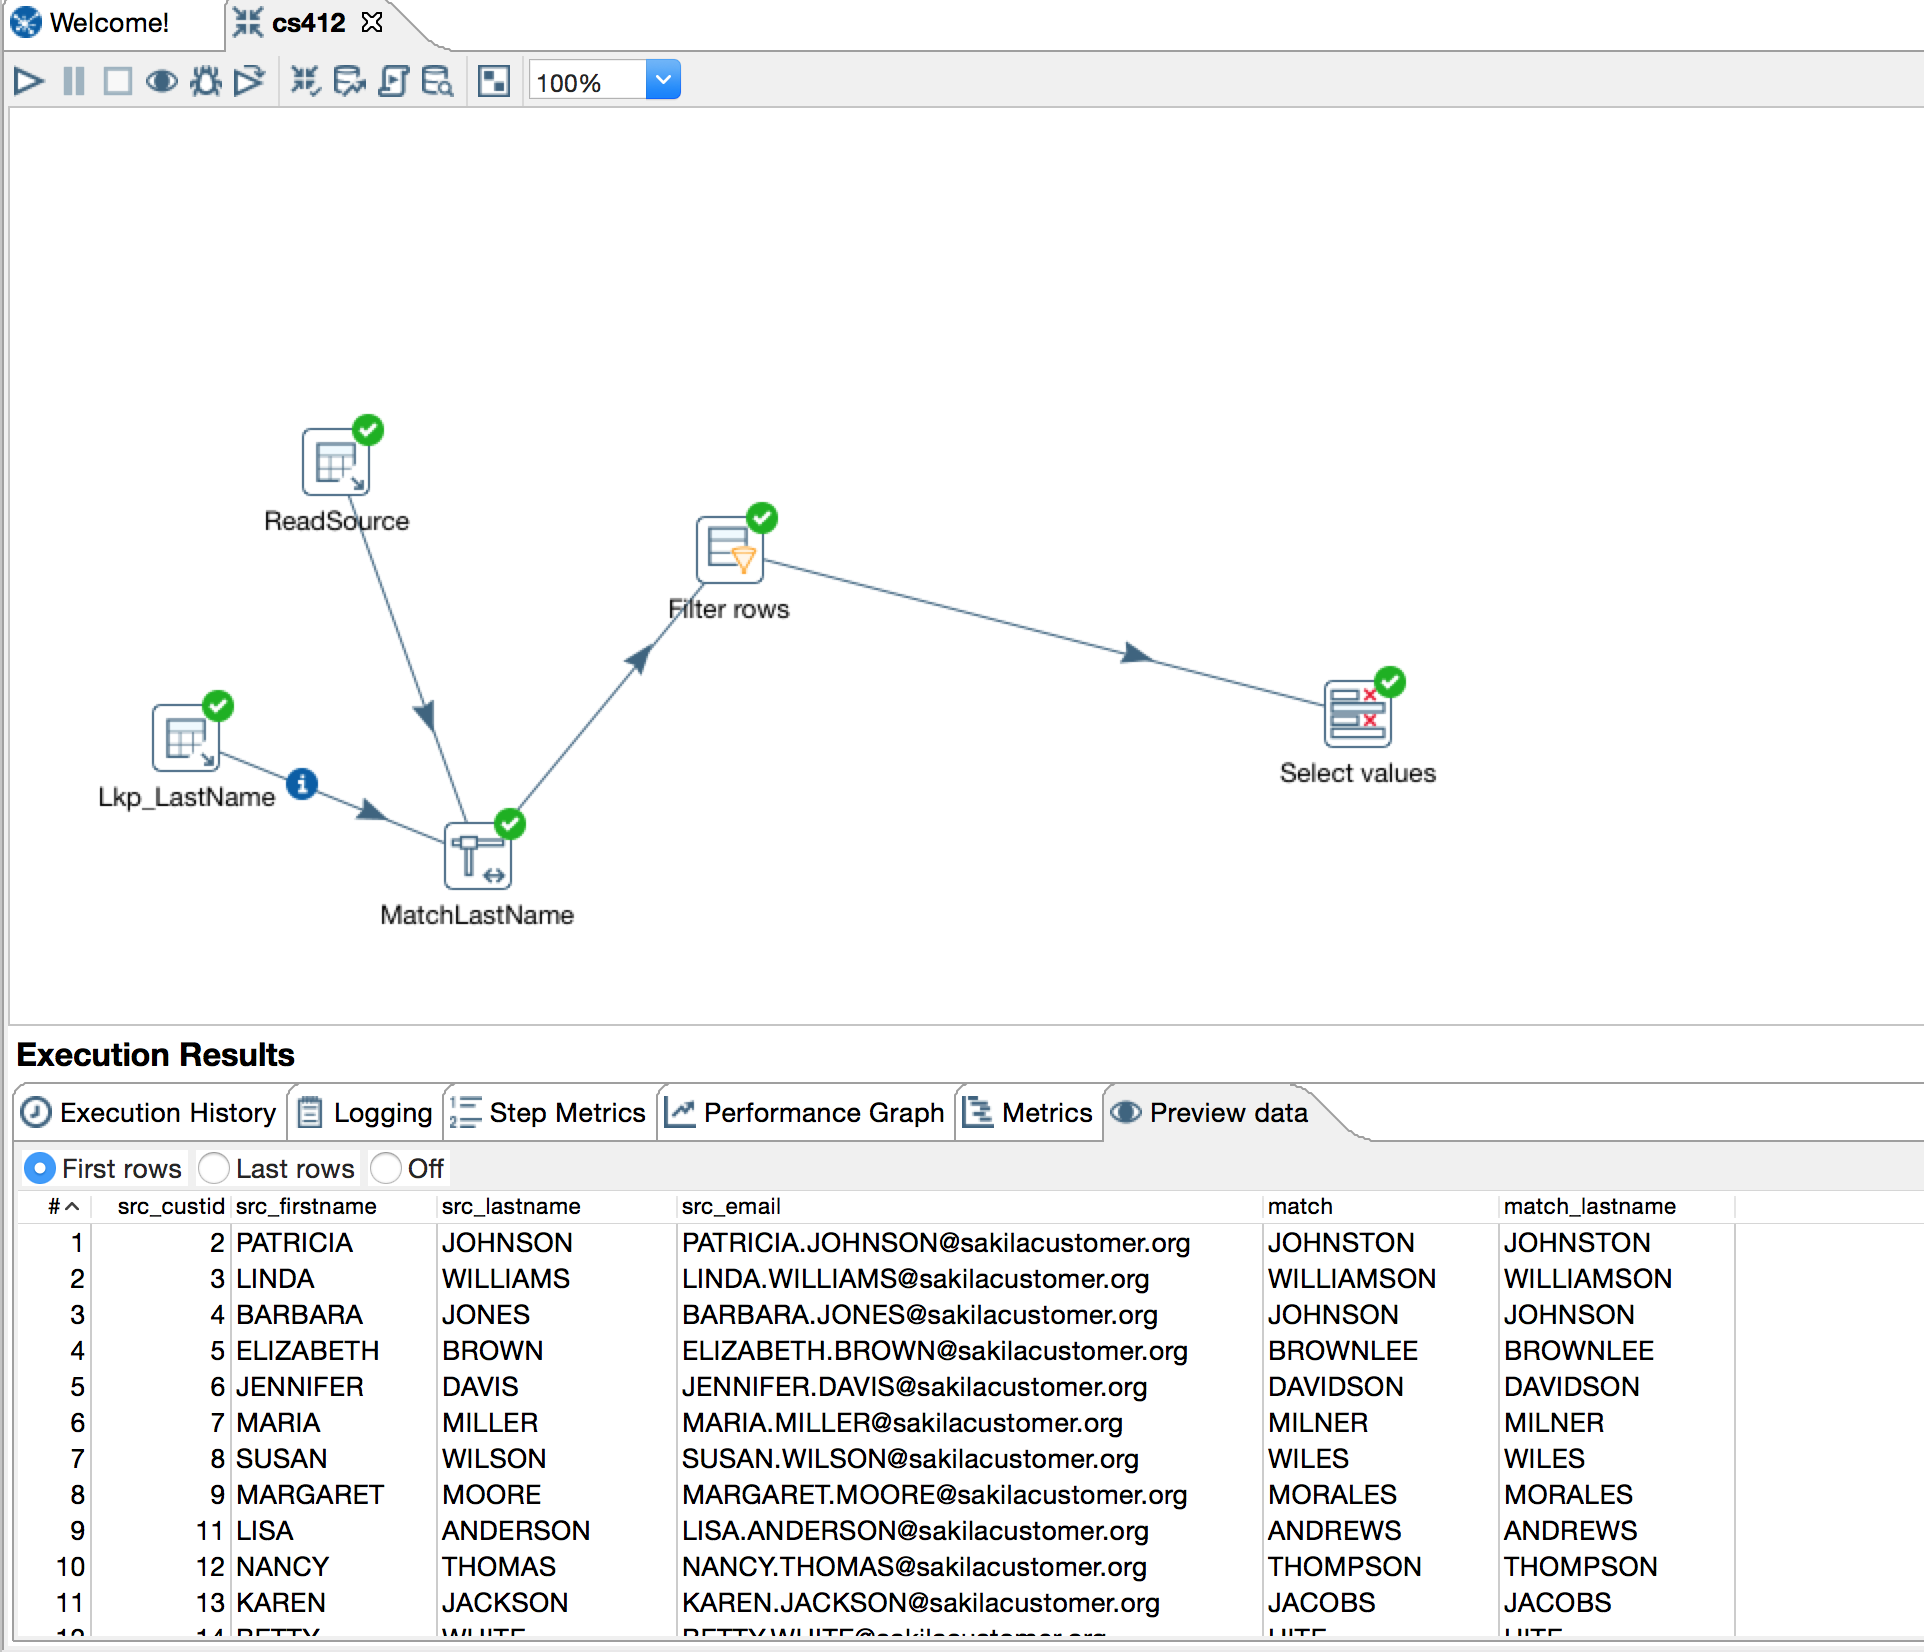
\includegraphics[width=10cm, height=10cm]{mp23}
  \end{figure}
\end{enumerate}